\section{Robust solution: SRP-PHAT}
\subsection{Behavior and error sources}
\subsubsection{Array response}
Beamforming techniques for sound localization have been study intensively over the last decades. The main drawback of the conventional beamforming are the side lobes in the localization results. If SRP-PHAT algorithm is applied to a tetrahedral array and cross-correlations values at different delays are summed by the beamformer (Eq. \ref{eq:srpSum}), subsidiary peaks can appear in the energy map at DOAs that don't correspond to the incident plane wave DOA. Those peaks in the SRP-PHAT energy map can mask real sources or even add up to other peaks from other sources, thus display a fake source. Deconvolution methods remove those peaks to reveal the correct peak. The algorithms for deconvolution are based on the point spread function, which is the response of the array to a point source. 
%For far-field, this means a plane wave incident with a particular DOA on the microphone array. In transfer function terms, the array response is `deconvolved' from the final energy map. 
%While this problem has motivated the creation of new beamformers {!!CITATION!!}, the problem lies in the method itself.
%New classes of algorithms have been developed to deconvolve the noise signals from the desired steered signal such as CLEAN \cite{sijtsma2007clean} and DAMAS \cite{brooks2006deconvolution}.
%DAMAS was acknowledged a major breakthrough in array processing. At first research was mainly focused on aeroacoustic for the development of near-field sound localization system but it seems that a new enthusiasm has taken over scientists trying to solve other sound localization problems. 
%While the DAMAS method is mainly designed for near field measurements in the range of the array aperture size, a new deconvolution method has been proposed [\cite{zhao2015large}, \cite{zhao2017large}] where a small aperture array is used to measure source signal in the far field. The principle behind point spread function is discussed in the following section. Then a review of the underlying principles of the main deconvolution algorithms is given, and finally a specific method for coherent and incoherent sources localization is discussed.
A perfect array will detect a point precisely at the actual source location and nothing elsewhere. This, however, is not the general case. For example, given a single pair of microphones, and assuming far-field incidence, the only information that can be concluded from a single point source is the angle of incidence on the array. This angle is a vector combination of source azimuth and elevation. This leads to a circle around the array where the source might be located (circular maximum peak). This circle is the base of the cone resulting from the cone approximation discussed previously.

%\begin{figure}[H]
%    \centering
%    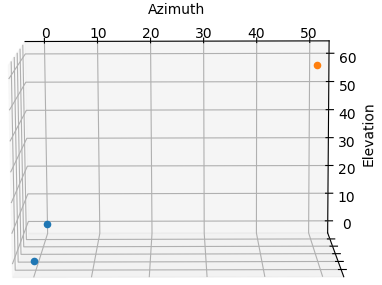
\includegraphics[width=0.98\textwidth]{Figures/2mic1src.png}
%    \caption{Figure depicts a source located at $50\degree$ azimuth and $60\degree$ elevation (orange dot). Two microphones (blue dots) will be used to localize the source.}
%    \label{fig:2mic1srcPos}
%\end{figure}

\begin{figure}[H]
    \centering
    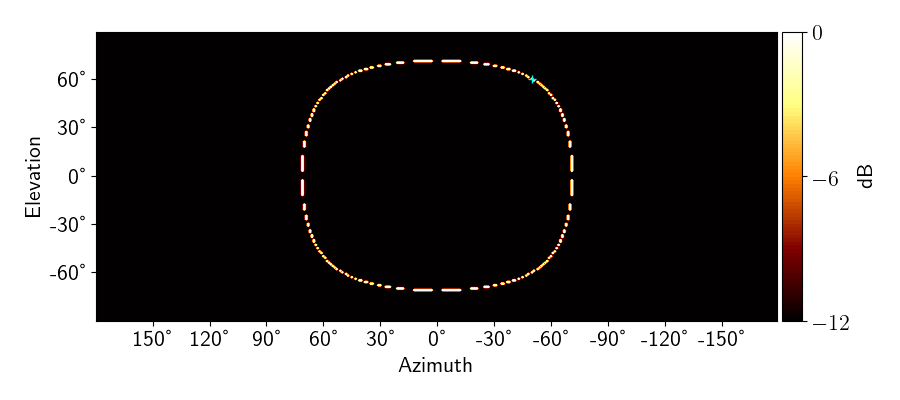
\includegraphics[width=0.8\textwidth]{Figures/2mic1srcRes.png}
    \caption{SRP-PHAT is run to localize a single point source with 2 microphones. The source is localized to a circle. The red dot indicates the actual source location.}
    \label{fig:2mic1src}
\end{figure}

If three microphones are placed in a horizontal equilateral triangle, we get three circles (three possible pairs of microphones) from localization. The maximum peak occurs at 2 locations with azimuth=50$\degree$ and elevation=$\pm 60\degree$.
\begin{figure}[H]
    \centering
    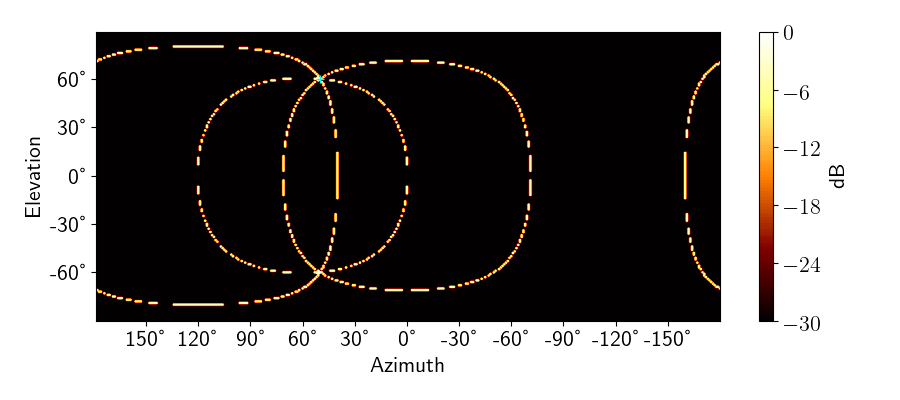
\includegraphics[width=0.8\textwidth]{Figures/3mic1srcRes.png}
    \caption{SRP-PHAT is run to localize the source with 3 microphones.}
    \label{fig:3mic1src}
\end{figure}

For a tetrahedral array, the point spread function is a combination of circles from the 6 possible microphone pairs. This time the main peak occurs at exactly one point. However, since only 3 pairs out of the 6 are linearly independent (Eq. \ref{Eq:linearDep}), the localization should really be done considering only 3 of those pairs. The result in shown in fig. \ref{fig:4mic1srcInd}
\begin{figure}[h]
    \centering
    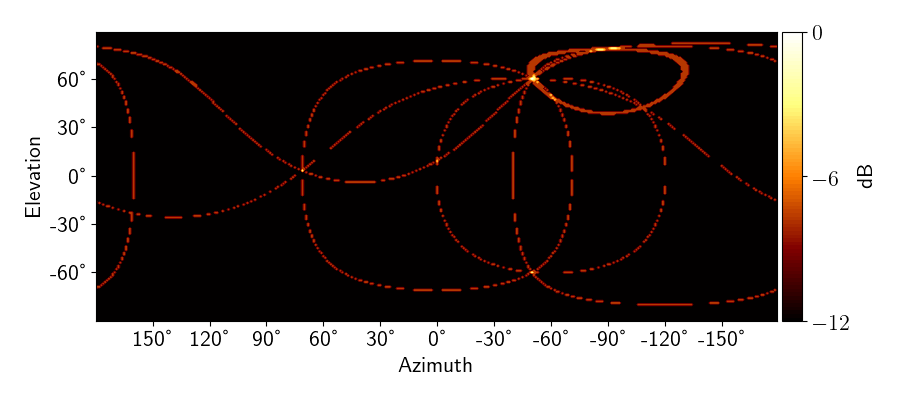
\includegraphics[width=0.8\textwidth]{Figures/4mic1srcRes.png}
    \caption{SRP-PHAT is run to localize the source with a tetrahedral array.}
    \label{fig:4mic1src}
\end{figure}


\begin{figure}[h]
    \centering
    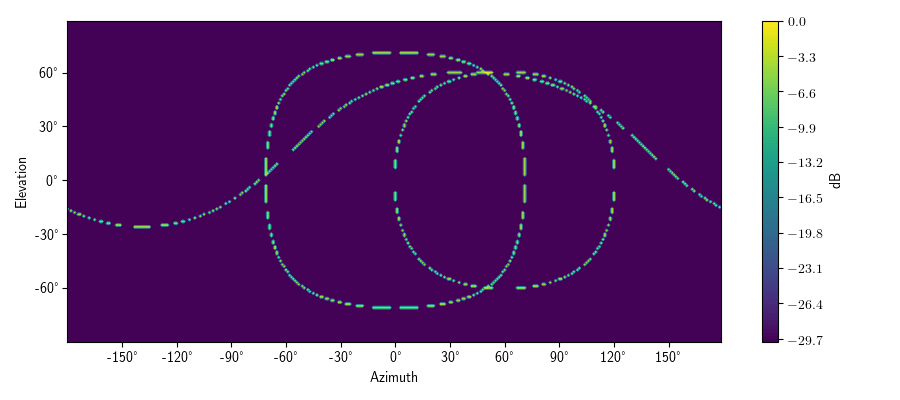
\includegraphics[width=0.8\textwidth]{Figures/Ind4mic1src.png}
    \caption{SRP-PHAT is run to localize the source with a tetrahedral array but only linearly independent microphone pairs are considered}
    \label{fig:4mic1srcInd}
\end{figure}
The result in fig. \ref{fig:4mic1src} is applicable only in ideal conditions (zero noise, no reflections and perfectly planar propagation). The localization result obtained in noisy conditions, is depicted in fig. \ref{fig:4mic1srcNoisy}. Note that the color bars for the figures depicted are of the same color scale. The localization performance deteriorates as the SNR drops. The result is similar to the results for PHAT with 2 microphones discussed earlier as the underlying process in SRP-PHAT is still PHAT. As can be seen in the figure, even in ideal conditions, the localization results contain many peaks of varying heights. This is due to summing the cross-correlation responses of a non-linear array (Eq. \ref{eq:srpSum}). If the array were linear, the localization circles from each pair would all overlap completely. In case of a tetrahedral array, the localization circles from the possible microphone pairs are not co-planar. This is because all the edges of a tetrahedron point in the different directions. The obvious problem here is multi-source detection. If multiple sources are playing at different levels, how do we determine if a detected peak is a real source or a relic from another higher level source? The methods to do so form the basis of deconvolution methods. A simple deconvolution approach could be to penalize sources detected only by a subset of the microphone pair combinations. This could be done by taking a product and not a sum in Eq. \ref{eq:srpSum}. This way, if a peak is caused by a single localization circle, the cross-correlation values from other microphone pairs would be close to zero, and thus would scale the false peak down. The localization results from this are given in fig. \ref{fig:4mic1srcNoisyProd}. Fig. \ref{fig:4mic2srcNoisyCompare} compares the localization result for two equally loud sources, this time located at (azimuth, elevation) = (-20, -30) and (50, 60), with normal SRP-PHAT and product-SRP-PHAT. The results are convincingly better for simulations.  

\begin{figure}[H]
    \centering
    \begin{subfigure}[b]{0.96\textwidth}
    \centering
    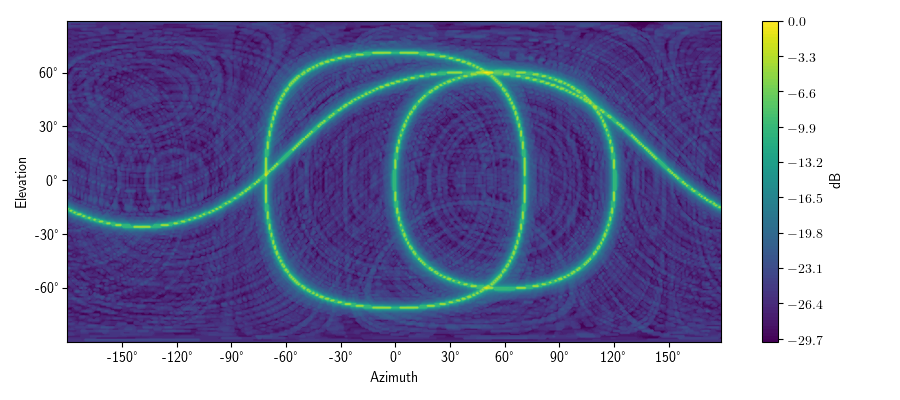
\includegraphics[width=0.8\textwidth]{Figures/Ind4mic1src20.png}
\end{subfigure}
\vskip \baselineskip
\begin{subfigure}[b]{0.96\textwidth}
    \centering
    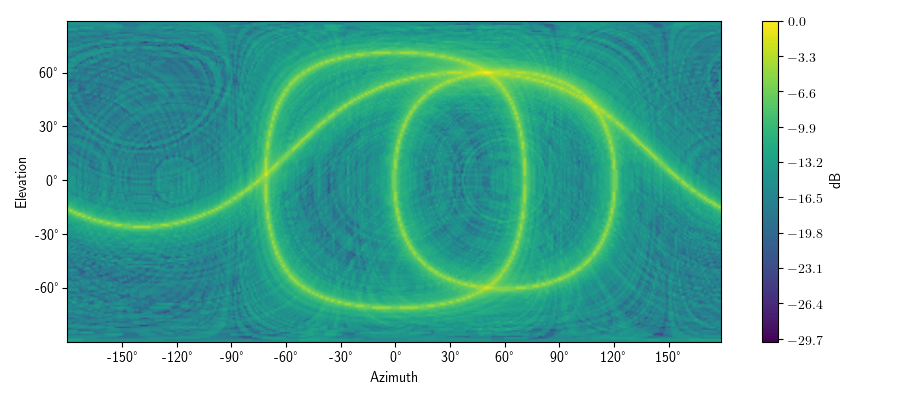
\includegraphics[width=0.8\textwidth]{Figures/Ind4mic1src6.png}
\end{subfigure}
\vskip \baselineskip
\begin{subfigure}[b]{0.96\textwidth}
    \centering
    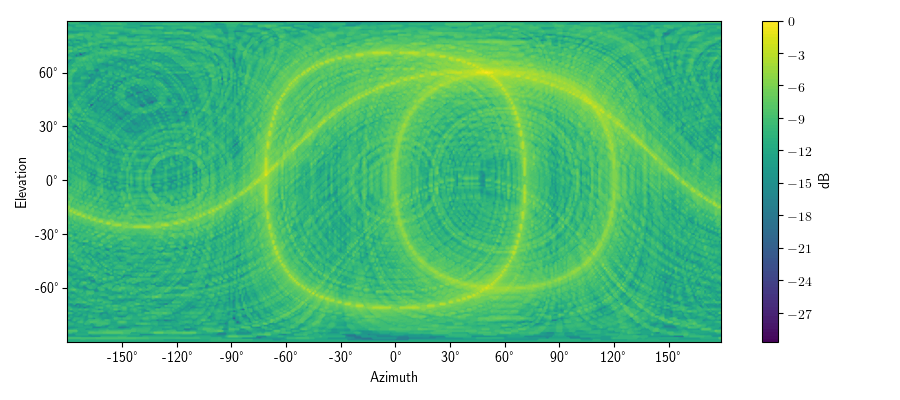
\includegraphics[width=0.8\textwidth]{Figures/Ind4mic1src0.png}
\end{subfigure}
\vskip \baselineskip
\begin{subfigure}[b]{0.96\textwidth}
    \centering
    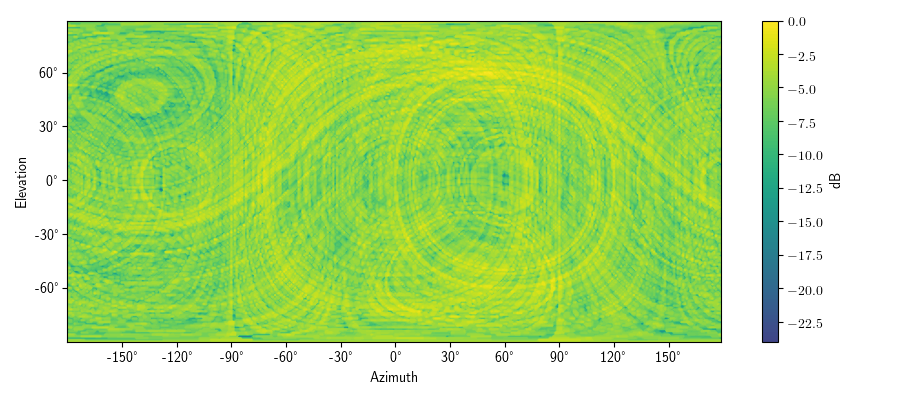
\includegraphics[width=0.8\textwidth]{Figures/Ind4mic1srcNeg6.png}
\end{subfigure}
\caption{Figures depict from top-to-bottom SRP-PHAT localization results with SNR = 20dB, SNR = 6dB, SNR = 0dB, SNR = -6dB}
\label{fig:4mic1srcNoisy}
\end{figure}

 \begin{figure}[H]
    \centering
    \begin{subfigure}[b]{0.96\textwidth}
    \centering
    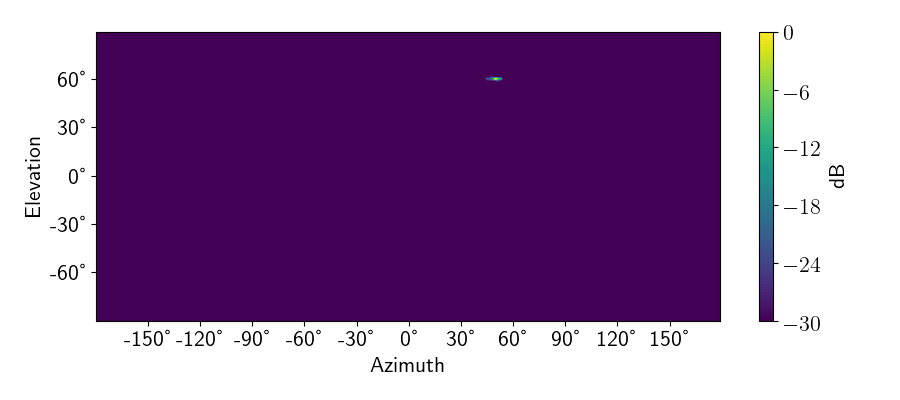
\includegraphics[width=0.8\textwidth]{Figures/Ind4mic1srcProd20.png}
\end{subfigure}
\vskip \baselineskip
\begin{subfigure}[b]{0.96\textwidth}
    \centering
    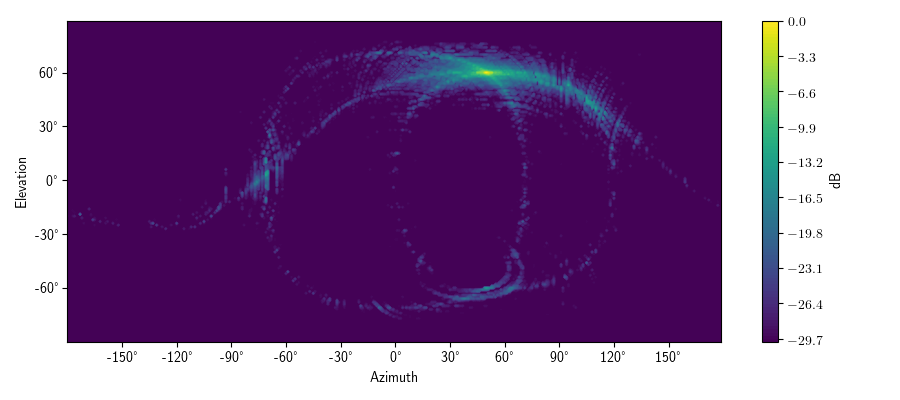
\includegraphics[width=0.8\textwidth]{Figures/Ind4mic1srcProd6.png}
\end{subfigure}
\vskip \baselineskip
\begin{subfigure}[b]{0.96\textwidth}
    \centering
    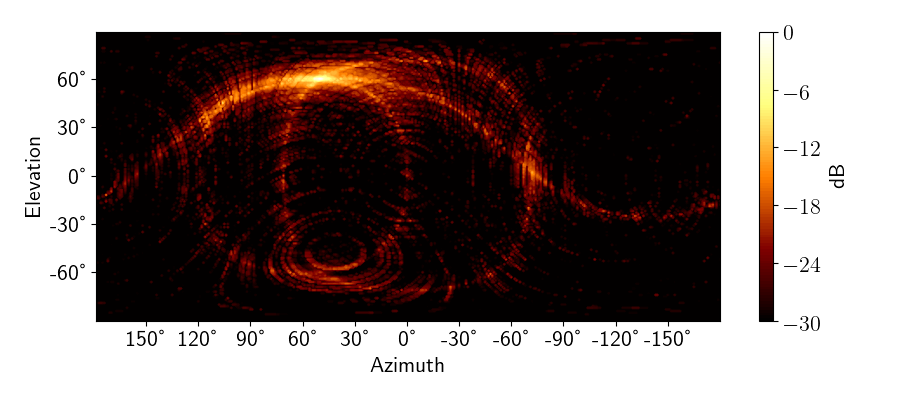
\includegraphics[width=0.8\textwidth]{Figures/Ind4mic1srcProd0.png}
\end{subfigure}
\vskip \baselineskip
\begin{subfigure}[b]{0.96\textwidth}
    \centering
    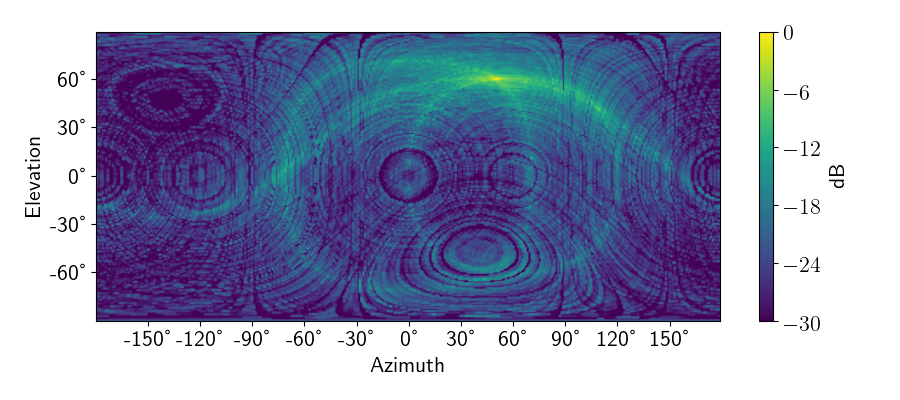
\includegraphics[width=0.8\textwidth]{Figures/Ind4mic1srcProdNeg6.png}
\end{subfigure}
\caption{Figures depict from top-to-bottom product-SRP-PHAT localization results  with SNR = 20dB, SNR = 6dB, SNR = 0dB, SNR = -6dB}
\label{fig:4mic1srcNoisyProd}
\end{figure}

 \begin{figure}[H]
    \centering
    \begin{subfigure}[b]{0.96\textwidth}
    \centering
    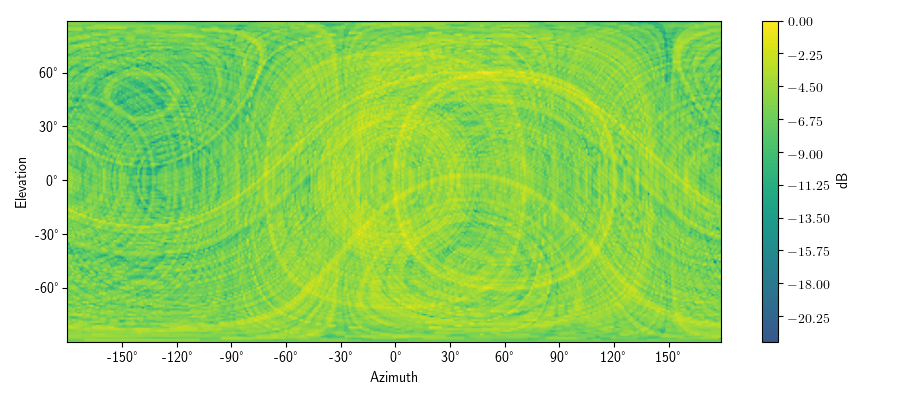
\includegraphics[width=0.8\textwidth]{Figures/Ind4mic2srcSumNeg6.png}
\end{subfigure}
\vskip \baselineskip
\begin{subfigure}[b]{0.96\textwidth}
    \centering
    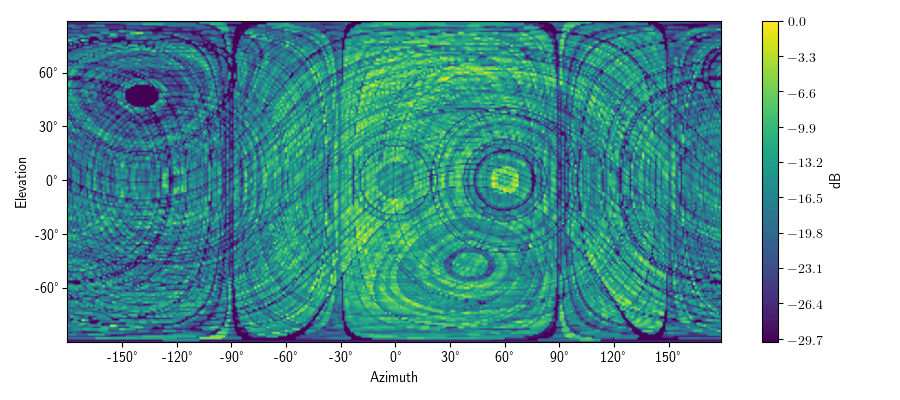
\includegraphics[width=0.8\textwidth]{Figures/Ind4mic2srcProdNeg6.png}
\end{subfigure}
\caption{Figures depict from localization results with normal SRP-PHAT (top) and product-SRP-PHAT (bottom)}
\label{fig:4mic2srcNoisyCompare}
\end{figure}

\begin{figure}[H]
    \centering
    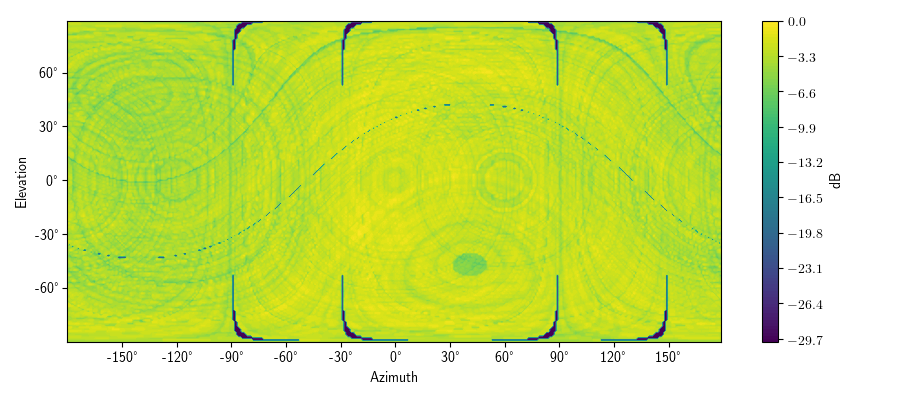
\includegraphics[width=0.8\textwidth]{Figures/Ind4mic2srcProdNeg6Div.png}
    \caption{Product-SRP-PHAT is run to localize 2 sources located at (azimuth, elevation) = (-20, -30) and (50, 60) with a tetrahedral array. The result is divided by 3 and normalized before visualization to maintain the level difference between the different sources.}
    \label{fig:4mic2srcNoisyDiv}
\end{figure}

The drawback of using product-SRP-PHAT is that the sound level difference between the different sound sources is lost. In normal SRP-PHAT, the array magnitude response at a particular azimuth and elevation could be averaged over all microphone pair combinations. Then the level difference between 2 sources is maintained. In product-SRP-PHAT this would not be the case. However if it is assumed that a particular source will have similar magnitude response for all microphone pairs (which is not a strong assumption in far-field), then taking the cubic root of multiplied power from the possible microphone pairs, the level difference can be maintained. When plotted on dB scale, that means a simple division by 3 depicted in fig. \ref{fig:4mic2srcNoisyDiv}. Since the division has the effect of reducing the dB difference between the noise floor and the main peak, the result deteriorates.

\begin{figure}[H]
    \centering
    \begin{subfigure}[b]{0.96\textwidth}
    \centering
    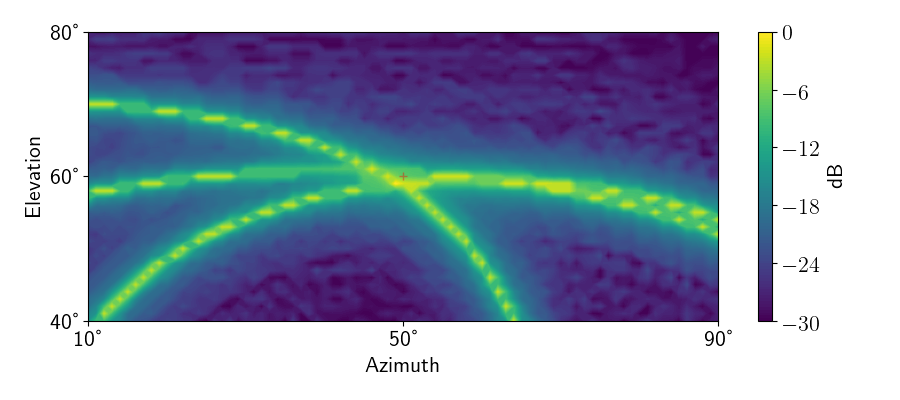
\includegraphics[width=0.8\textwidth]{Figures/Ind4mic1srcSum0deg.png}
\end{subfigure}
\vskip \baselineskip
\begin{subfigure}[b]{0.96\textwidth}
    \centering
    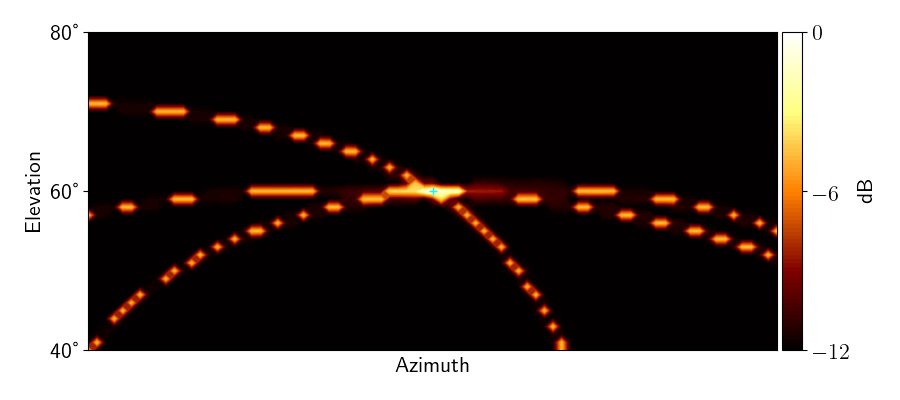
\includegraphics[width=0.8\textwidth]{Figures/Ind4mic1srcSum20deg.png}
\end{subfigure}
\vskip \baselineskip
\begin{subfigure}[b]{0.96\textwidth}
    \centering
    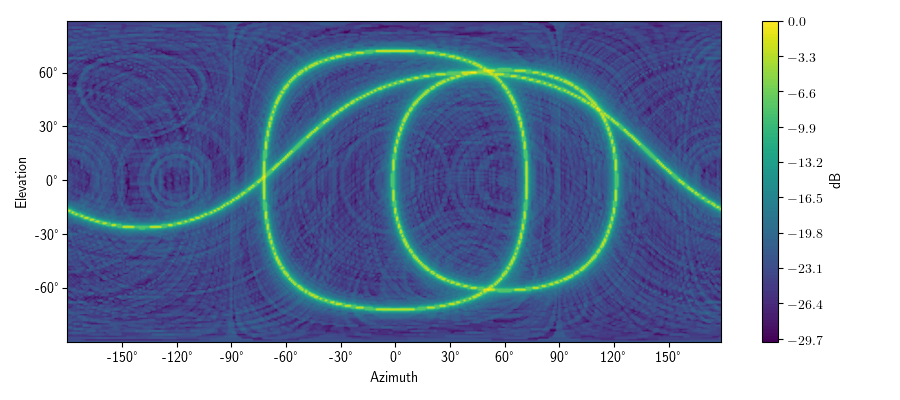
\includegraphics[width=0.8\textwidth]{Figures/Ind4mic1srcSum40deg.png}
\end{subfigure}
\caption{Figures depict from top-to-bottom SRP-PHAT localization results with at temperatures of $0\degree C$, $20\degree C$ and $40\degree C$. SNR = 20dB for every case.}
\label{fig:4mic1srcTemp}
\end{figure}

\subsubsection{Effect of temperature}
Temperature affects the speed of sound and thus affects the delay time between the microphone pairs. During measurement, if it is assumed to be room temperature, this could lead to errors in the localization results. Fig.\ref{fig:4mic1srcTemp} depicts the effect of temperature on localization results, where wave files received by the tetrahedral microphone array at temperatures of $0\degree C$, $20\degree C$ and $40\degree C$ are simulated. Then the localization is run assuming the speed of sound to be 343m/sec in every case. As can be seen in the figure, an error in recording temperature has the effect of `de-focusing' the main peak. This could lead to even great localization errors if naive deconvolution algorithms (like the product-SRP-PHAT) are then directly applied to the result. 

\begin{figure}[H]
    \centering
    \begin{subfigure}[b]{0.96\textwidth}
    \centering
    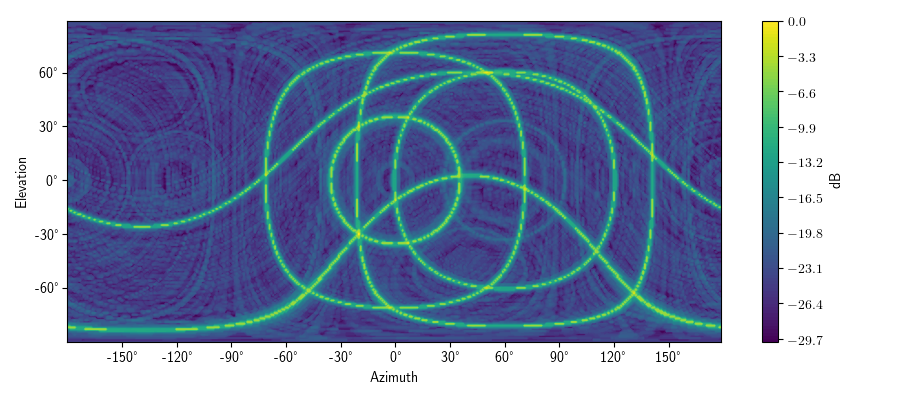
\includegraphics[width=0.8\textwidth]{Figures/Ind4mic1srcSumWind0.png}
\end{subfigure}
\vskip \baselineskip
\begin{subfigure}[b]{0.96\textwidth}
    \centering
    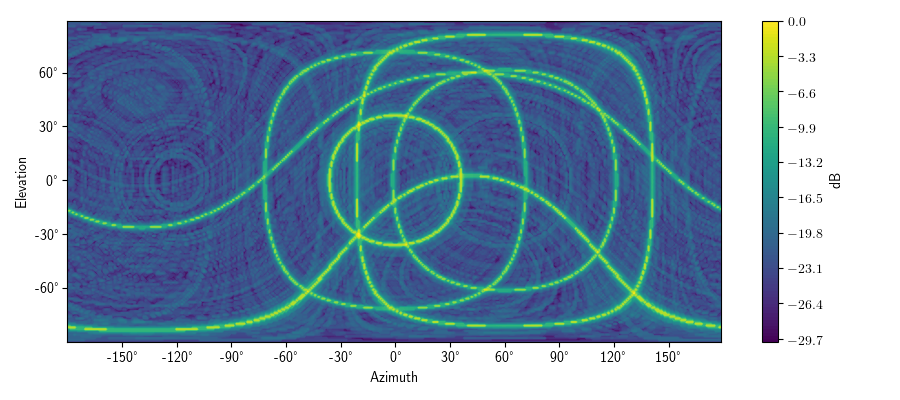
\includegraphics[width=0.8\textwidth]{Figures/Ind4mic1srcSumWind10.png}
\end{subfigure}
\vskip \baselineskip
\begin{subfigure}[b]{0.96\textwidth}
    \centering
    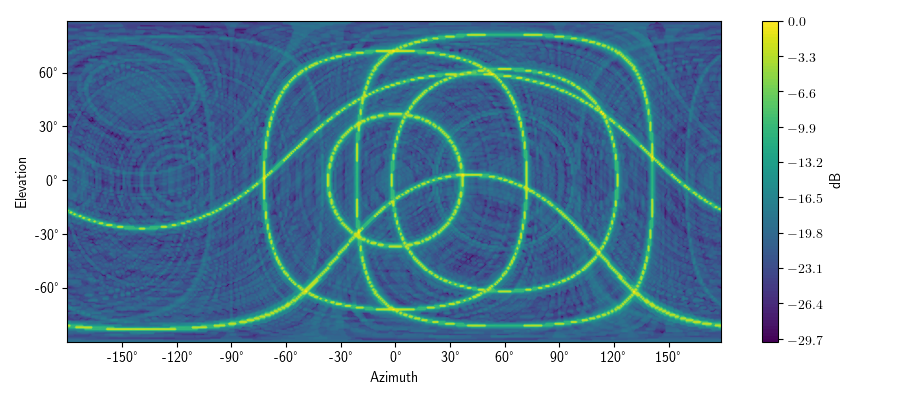
\includegraphics[width=0.8\textwidth]{Figures/Ind4mic1srcSumWind20.png}
\end{subfigure}
\caption{Figures depict from top-to-bottom SRP-PHAT localization results with wind of $0 m/sec$, $10 m/sec$ and $20 m/sec$. 2 sources located at (azimuth, elevation) = (-20, -30) and (50, 60) are localized with at wind (azimuth,elevation) = (50,0) and SNR = 20dB for every case.}
\label{fig:4mic2srcWind}
\end{figure}

\subsubsection{Effect of wind}
Wind speed effects the speed of sound in the direction of propagation. Delays between different array pairs would be affected depending on where the SRP search is looking and from what direction the wind is blowing. If wind blows perpendicular to the direction of propagation of the sound from the source, then it does not affect the localization. In case of multiple sources, the extent of errors due to wind will depend on the source location. Assuming wind to be blowing level (horizontally), wind direction can be described by its magnitude in m/sec and its azimuth. Fig.\ref{fig:4mic2srcWind} depicts the effect when localizing two equally loud sources without any wind correction, located at (azimuth, elevation) = (-20, -30) and (50, 60) for various conditions.

\subsubsection{Effect of ground reflections}
Sound received from a far-field sound source consists of the plane wave and the spherical wave component (Eq. \ref{Eq:GroundWave}). The plane wave components is the only component simulated so far above. The ground wave which is the spherical wave component needs to be considered as well. It is the contribution of the image created by the source with the ground. The location of this reflected sound is in vicinity of the image and depends on the smoothness of the ground material. Its magnitude depends on the magnitude of absorption of sound by the ground. Rudimentary simulations for a source located at $(\theta,\phi)$ can be made assuming sound sources located at $(\theta,-\phi)$ and $(\theta,0)$. Fig. \ref{fig:4mic1srcRef} shows the localization results with the same source located at those locations. More complex reflections are not currently planned for simulation purposes.

\begin{figure}[H]
    \centering
    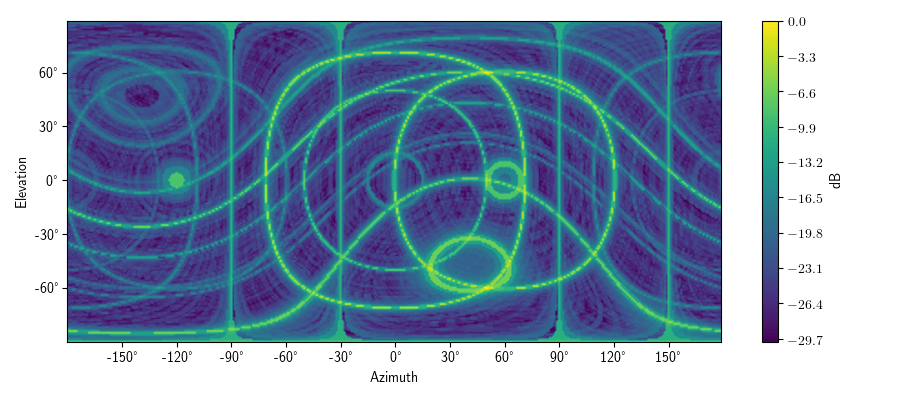
\includegraphics[width=0.8\textwidth]{Figures/Ind4mic1srcSumRef.png}
    \caption{SRP-PHAT is run to localize a source located at (azimuth, elevation) = (50, 60). The source is also copied at locations (50,0) and (50,-60).}
    \label{fig:4mic1srcRef}
\end{figure}